\pagestyle{fancy}
\headheight 20pt
\lhead{Ph.D. Thesis --- R. Woods}
\rhead{McMaster - Physics \& Astronomy}
\chead{}
\lfoot{}
\cfoot{\thepage}
\rfoot{}
\renewcommand{\headrulewidth}{0.1pt}
\renewcommand{\footrulewidth}{0.1pt}

\chapter{Introduction}
\label{chap:intro} 
\thispagestyle{fancy} 

It doesn't take much to convince a physicist of the importance of photons - astrophysical objects ``speak'' in photons. As astronomers, we receive all of our information in the universe through photons. In order to understand the objects we observe, we must understand photons and the physical processes that tie them to matter. 

\section{The Role of Radiation in Astrophysics}
\label{sec:radinastro}

When considering galaxies, for example, many of the galaxy properties are determined by the stars inside of it and the gas and dust between those stars. The rate at which a galaxy forms stars is dependent on the state of the gas, which is largely dependent on the Interstellar Radiation Field (ISRF), which is in turn dependent on the surrounding stars \citep{leithererEt99}. While gas can be heated by other sources than the ISRF such as gravitational heating, for the purpose of this thesis, we focus on the ISRF, which has been shown to dominate for gas phased less than $1\e{4} K$ \citep{wolfireEt03}.

In order to form stars, gas must be at low temperatures and high densities. This means gas cooling must be high compared to heating due to the ISRF. Cooling rates depend on the species present in the gas and the processes that are removing energy. Important processes include line cooling, including metal lines, bremsstrahlung radiation, thermal emission from dust grains, and thermal x-ray emission. Many of the photons emitted in the above fashion can also act to heat the gas if the gas temperature is lower than the energy associated with the incident photons. Other heating sources include stellar emission, photoelectric heating, and (although they're not photons), cosmic rays.

If photon energies are higher than the binding energy of electrons in gas or dust, then electrons can be freed. In the case of atoms, this causes (photo) ionization. In the case of dust, it causes the dust grains to become negatively charged and the freed electrons to be available for photoelectric heating. In the case of molecules, the molecule can be dissociated.

Photoionization is most common with the most abundant gas elements, Hydrogen. This requires photons more energetic than 13.6 ev corresponding to the Extreme Ultraviolet (EUV) part of the spectrum. Near massive O and B stars, which emit heavily in the UV, these photons cause large ionized regions of Hydrogen, or HII regions. However, because these photons are so readily absorbed, they are largely absent from regions further from stars. Photons at energies higher than 13.6 ev not only ionize the atoms, but impart kinetic energy to the ejected electrons, which in turn heats the gas to average temperatures of 25,000 K.

\begin{figure}
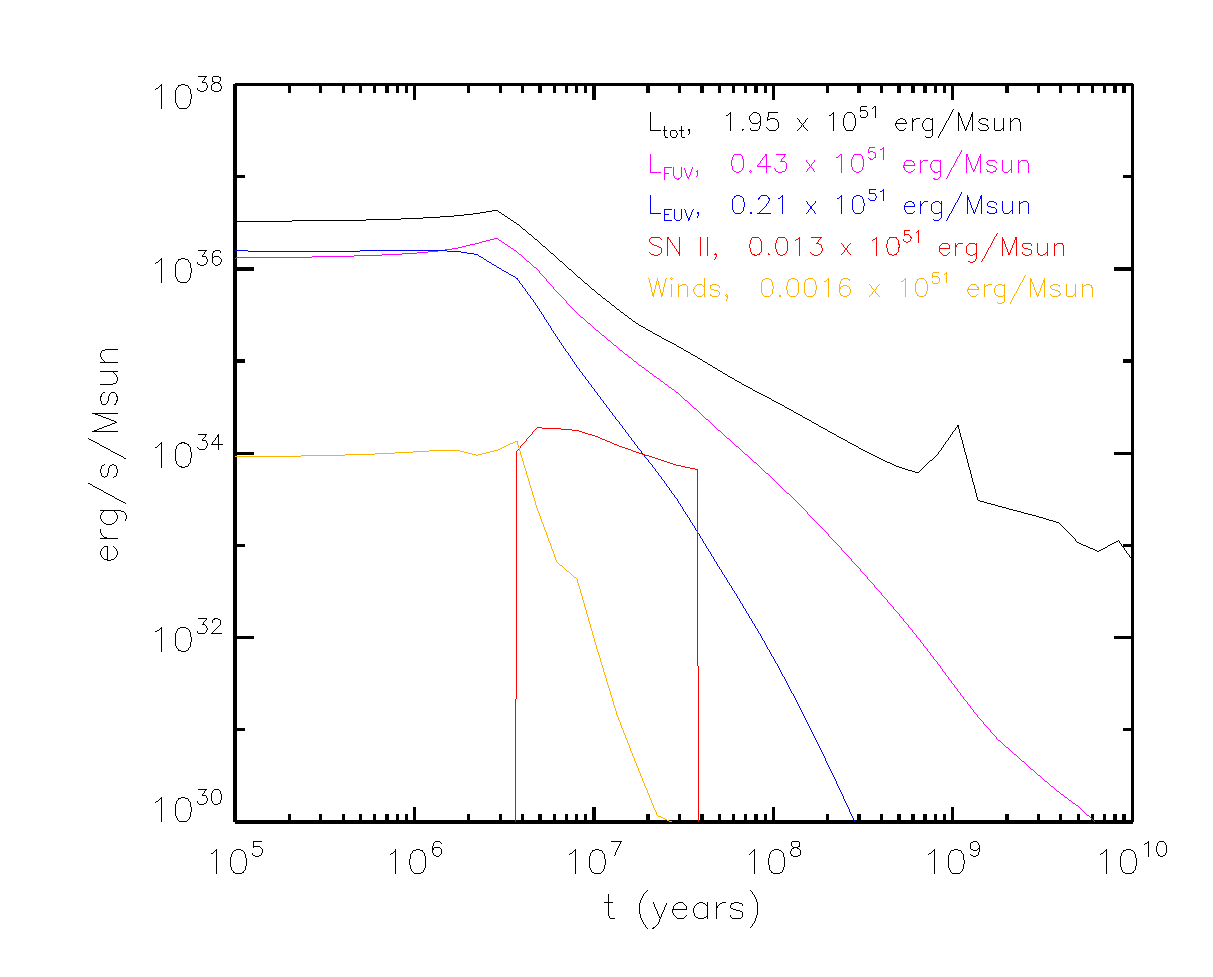
\includegraphics[width=\textwidth]{graphics/UVSN.eps}
\caption[Energy available per band.]{Cumulative energy vs time available from a star cluster for different energy bands.}
\label{fig:bandenergies}
\end{figure}

In neutral regions where no H-ionizing photons are present, ionization of other elements become important. Due to Carbon's high abundance, it becomes the dominant heating mechanism. The energy needed to ionize Carbon is 11.3 ev, so photons between 11.3 ev and 13.6 ev become an important source of heating. 

Below 11.3 ev, the Far Ultra Violet (FUV) spectrum becomes important. Photons in this part of the spectrum are typical of large B stars, and while they don't have enough energy to ionize Hydrogen, they do have enough to free electrons from dust and Polycyclic Aromatic Hydrocarbon (PAH) molecules and impart kinetic energy to the freed electron. This drives one of the most important heating mechanisms in Interstellar Medium (ISM), photoelectric heating.

At energies much lower than FUV, photons become a a less important factor to heating and tend to act more as cooling mechanisms. Emission in the Infrared (IR) is especially common for dust cooling due to blackbody radiation.

Further sources of heating can be found at higher energies in X-rays, which have large energies but low intensity. X-rays become an important heating mechanisms for warm, low density, neutral gas.

%\begin{itemize}
%\item ISM
%\begin{enumerate}
%  \item photoelectric (PE)
%  \item cosmic rays (CR)
%  \item Carbon I (CI)
%\end{enumerate}
%\item Warm Neutral Medium
%\begin{enumerate}
%  \item CR/PE
%  \item X-rays
%\end{enumerate}
%\item Molecular Clouds
%\begin{enumerate}
%\item Cosmic Rays
%\item Turbulence
%\item Dust + gas
%\end{enumerate}
%\end{itemize}

Even with this very limited overview of heating and cooling, it becomes abundantly clear how important radiation is in determining the state of astronomical material. If we are to simulate the Universe, then we must properly capture the behavior of radiative transfer.

%
%\begin{itemize}
%\item Introduce stellar systems -  radiation can provide pressure support, can cause ionization, dissociation, can heat the gas. Because gas properties tied to star formation rate, and stars are one of the primary targets of observation, it's important to know what's going on.
%\item Introduce cosmology (how in depth here?). Cosmology depends on knowing photon history and what cosmological factors affect photons. Introduce cosmic reionization, Universe expansion, SZ?, lensing?, CMB?
%\item Need to ability to track photoionization, photoheating across huge amounts of sources and their environments. Astrophysical radiation has both short and large scale effects that can't be ignored.
%\end{itemize}

%[abelnormanmadau has good cosmo-intro w/ references.]


%Introduction to the basics of cosmology
%·         properties in the context of computational radiative transfer
%
%·         important evends like re-ionization of the universe
%
%·         ionization fronts and large numbers of sources
%
%·         with a focus on the physics side of things
%
% 
%Astro relies on photons - language of the universe
%·         only way the universe can be observe
%
%·         needs to be understood to get an idea of how things are interacting
%
% 
%Look at cosmology and stellar systems where these things are really important. 
%·         In order to understand why the algorithm needs to function the way it does, need to understand cosmology to have relevant applications
%
%·         Need to develop a what to represent approximations to deal with the large length scales and large number of sources.


%First part - what is this document? What will be in it? What is the main thing I will be telling you about? [Move this after intro to astro stuff? I think so...].



\section{Overview}
\label{sec:overview}

Chapter \ref{chap:radtransfer} will go over the background of radiative transfer and the currently available codes that solve the radiative transfer problem. It will also motivate the need for a new code in a particular niche. Chapter \ref{chap:method} will introduce the new radiative transfer method that we have developed. Chapter \ref{chap:codetests} will demonstrate the strengths and weaknesses of the new algorithm through a variety of numerical and phyical tests. Chapter \ref{chap:galaxyformation} will show the results of using the algorithm on an isolated galaxy in the FUV band, and will also focus on future projects that the algorithm will be used for. Finally, chapter \ref{chap:conclusions} contains the conclusions of this thesis.
